\documentclass[a4paper,11pt]{article}
\usepackage[table]{xcolor}



\newcommand{\defeq}{\mathrel{\doteq}}

\newcommand{\lzero}{0}

\newcommand{\kw}[1]{\mathtt{#1}}

\newcommand{\expr}{e}
\newcommand{\vall}{w}
\newcommand{\valr}{v}
\newcommand{\eif}{\kw{if}}
\newcommand{\eapp}{\;}
\newcommand{\eprojl}{\kw{fst}}
\newcommand{\eprojr}{\kw{snd}}
%\newcommand{\eprov}[1]{\eta_{#1}}
\newcommand{\etrue}{\kw{true}}
\newcommand{\efalse}{\kw{false}}
\newcommand{\econst}{c}
\newcommand{\eop}{\delta}
\newcommand{\efix}{\mathop{\kw{fix}}}
%\newcommand{\labelA}{\ell}

\newcommand{\tr}{T}
\newcommand{\trift}{\eif^{\kw{t}}}
\newcommand{\triff}{\eif^{\kw{f}}}
\newcommand{\trprojl}{\eprojl}
\newcommand{\trprojr}{\eprojr}
\newcommand{\trtrue}{\etrue}
\newcommand{\trfalse}{\efalse}
\newcommand{\trconst}{\econst}
\newcommand{\trop}{\eop}
\newcommand{\trfix}{\efix}
\newcommand{\trapp}[5]{#1 \; #2 \mathrel{\triangleright} {\efix #3(#4).#5}}

\newcommand{\adap}{\kw{adap}}
\newcommand{\ddep}[1]{\kw{depth}_{#1}}
\newcommand{\nat}{\mathbb{N}}
\newcommand{\natb}{\nat_{\bot}}
\newcommand{\natbi}{\natb^\infty}
\newcommand{\nnatA}{n}
\newcommand{\nnatB}{m}
\newcommand{\nnatbA}{s}
\newcommand{\nnatbB}{t}
\newcommand{\nnatbiA}{q}
\newcommand{\nnatbiB}{r}

\newcommand{\type}{\tau}
\newcommand{\tbase}{\kw{b}}
\newcommand{\tbool}{\kw{bool}}
\newcommand{\tarr}[5]{#1; #3 \xrightarrow{#4; \, #5} #2}
\newcommand{\env}{\theta}

\newcommand{\bigstep}{\mathrel{\Downarrow}}

\newcommand{\dmap}{\rho}
\newcommand{\dmapb}{\bot_\dmap}
\newcommand{\supp}{\kw{supp}}
\newcommand{\dom}{\kw{dom}}

\newcommand{\tvdash}[1]{\vdash_{#1}}

%Packages
\usepackage[T1]{fontenc}
\usepackage{fourier} 
\usepackage[english]{babel} 
\usepackage{amsmath,amsfonts} 
\usepackage{amsthm} 
\usepackage{color}   %May be necessary if you want to color links
\usepackage{hyperref}
\usepackage{lscape}
\usepackage{geometry}
\usepackage{amsmath}
\usepackage{algorithm}
\usepackage{algorithmic}
\usepackage{amssymb}
\usepackage{amsfonts}
\usepackage{times}
\usepackage{bm}
\usepackage{ stmaryrd }
\SetSymbolFont{stmry}{bold}{U}{stmry}{m}{n}

\usepackage{ amssymb }
\usepackage{ textcomp }
\usepackage[normalem]{ulem}
% For derivation rules
\usepackage{mathpartir}
\usepackage{color}
\usepackage{a4wide}
\usepackage{caption}
\usepackage{subcaption}
\usepackage{mathpartir}
\usepackage{amsmath,amsfonts}
\usepackage{ amssymb }
\usepackage{color}
\usepackage{algorithm}
\usepackage{algorithmic}
\usepackage{microtype}
\usepackage{eucal}
\usepackage{url}
\usepackage{xspace}
\usepackage{array}
\usepackage{listings}

\usepackage{tikz}
\usetikzlibrary{shapes.geometric}
\usetikzlibrary{arrows.meta,arrows}
\usetikzlibrary{decorations.text}
% % % % 


\usepackage{multirow}


%%%%%%%%%%%%%%%%%%%%%%%%%%%%%%%%%%%%%%%%%%%%%%%%%%%%%Packages And Definitions For Listing the Code%%%%%%%%%%%%%%%%%%%%%%%%%%%%%%%%%%%%%%%%%%%%%%%%%%%%%%%%%%%%%%%%%%%%%%%%
\usepackage{listings}
\usepackage{xcolor}

\definecolor{codegreen}{rgb}{0,0.6,0}
\definecolor{codegray}{rgb}{0.5,0.5,0.5}
\definecolor{codepurple}{rgb}{0.58,0,0.82}
\definecolor{backcolour}{rgb}{0.95,0.95,0.92}

\lstdefinestyle{mystyle}{
    backgroundcolor=\color{backcolour},   
    commentstyle=\color{codegreen},
    keywordstyle=\color{magenta},
    numberstyle=\tiny\color{codegray},
    stringstyle=\color{codepurple},
    basicstyle=\ttfamily\footnotesize,
    breakatwhitespace=false,         
    breaklines=true,                 
    captionpos=b,                    
    keepspaces=true,                 
    numbers=left,                    
    numbersep=5pt,                  
    showspaces=false,                
    showstringspaces=false,
    showtabs=false,                  
    tabsize=2
}

\lstset{style=mystyle}

\usepackage{tikz}
\usetikzlibrary{shapes,arrows}
\newcommand{\THESYSTEM}{\textsf{AdaptFun}}

% Define block styles
\tikzstyle{decision} = [diamond, draw, fill=blue!20, 
    text width=4.5em, text badly centered, node distance=3cm, inner sep=0pt]
\tikzstyle{block} = [rectangle, draw, fill=blue!20, 
    text width=5em, text centered, rounded corners, minimum height=4em]
\tikzstyle{line} = [draw, -latex']
\tikzstyle{cloud} = [draw, ellipse,fill=red!20, node distance=3cm,
    minimum height=2em]

\begin{document}
\title{Adaptivity Analysis}

\author{}

\date{}

\maketitle

\begin{abstract}
  A data analysis is said to \emph{generalize} when it allows one to draw
  conclusions from the data that are true of the population from which
  the data are sampled. Statistician and data scientist have devised
  several methods aimed to guarantee generalization in  data
  analyses, and avoid in this way overfitting to the
  data. Guaranteeing generalization is more difficult when data
  analyses are \emph{adaptive}: when the result of an analysis depends
  on the result of previous analyses. 

  A recent line of work focuses on methods aimed at guaranteeing
  generalization in adaptive data analysis through the addition of
  carefully calibrated statistical noise to the empirical results of
  the analysis on the sampled data. In these works, the confidence
  intervals on the generalization error that one can achieve for a
  given analysis usually depend on the \emph{level of adaptivity} of
  the analysis: the number of adaptive steps that depend on
  each other. 

  In this work we introduce a programming framework, named \THESYSTEM,  aimed at
  supporting the study of the generalization error for adaptive data
  analysis. Through its analysis system, an upper bound on the
  adaptivity -- depth (the length of the longest chain of queries) of
  a program implementing an adaptive data analysis can be overestimated. We show how this language can help to analyze the generalization error between two data analyses with different adaptivity structures.
\end{abstract}

\tableofcontents


% \section{Introduction}
\section{System Overview}
In adaptive data analysis, a data analysis can depend on the results of
previous analysis over the same data. This dependency may affect the
\emph{generalization properties of the data analysis}. To study this phenomenon
in a formal way, we consider the \emph{statistical query
  model}. In this model, a dataset $X$ consisting of $d$ attributes (columns) and $n$
individuals' data (rows) can be accessed only through an interface to
which one can submit statistical queries. More precisely, suppose that
the type of a row is $R$ (as an example, a row with $d$ binary
attributes would have type $R=\{0,1\}^d$. Then, in the statistical
query model one can access the dataset only by submitting a query to
the interface, in
the form of a function
$p:D\to [0,1] $ where $D$ represents dataset. The collected answer of
the asked query is the average result of $p$ on each row in the
dataset $D$. For example, the result is the
value $\frac{1}{n}\sum_{i=1}^n p(X_i)$ where
$X_i$ is the row of index $i$ in $X$. While this model is rather
simple, in fact it supports sufficient statistics one may be
interested.

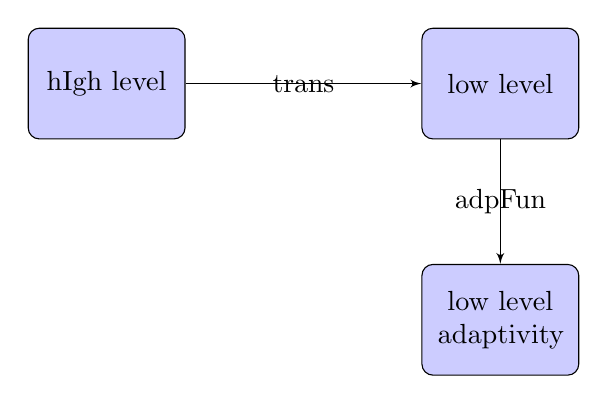
\begin{tikzpicture}{node distance = 2cm, auto}
  % nodes
  \node [block](high){hIgh level } ;
  \node [block, right of = high, node distance = 5cm](low){low level  } ;
  \node [block, below of = low, node distance = 3cm](adaptlow){low level adaptivity};
  % edges
  \path [line] (high) -- node {trans} (low) ;
  \path [line] (low) -- node {adpFun}(adaptlow);
 \end{tikzpicture} 

% \begin{tikzpicture}[node distance = 2cm, auto]
%     % Place nodes
%     \node [block] (init) {initialize model};
%     \node [cloud, left of=init] (expert) {expert};
%     \node [cloud, right of=init] (system) {system};
%     \node [block, below of=init] (identify) {identify candidate models};
%     \node [block, below of=identify] (evaluate) {evaluate candidate models};
%     \node [block, left of=evaluate, node distance=3cm] (update) {update model};
%     \node [decision, below of=evaluate] (decide) {is best candidate better?};
%     \node [block, below =decide, node distance=3cm] (stop) {stop};
%     % Draw edges
%     \path [line] (init) -- (identify);
%     \path [line] (identify) -- (evaluate);
%     \path [line] (evaluate) -- (decide);
%     \path [line] (decide) -| node [near start] {yes} (update);
%     \path [line] (update) |- (identify);
%     \path [line] (decide) -- node {no}(stop);
%     \path [line,dashed] (expert) -- (init);
%     \path [line,dashed] (system) -- (init);
%     \path [line,dashed] (system) |- (evaluate);
%   \end{tikzpicture}
 

We support the model by providing a ``high'' level language, which is
expressive to represent the adaptive mechnisms. In this language, the
queries are allow to carry arguments, for example, the expression
$q(e)$ simulates the process of submitting a query to the interface in
the model while the argument $e$ is consumed to construct the
query. For instance, one submitted query may use the average of
answers of previous queries, can be expressed $q(x)$ where $x$ stores
the expected average results in our language. In this sense,the result of the query from a specific $D$ can vary under different contexts.

Nevertheless, in \emph{statistical query
  model}, the dependency between two submitted queries is vague, especially when
we study in adaptive scenarios. Our definition of the dependency lies
in the independence between two queries: one query
$q_1$ does not
depend on another query $q_2$ when the result of $q_1$ remains the
same regardless of the modification of the result of $q_2$. Following such
definition, the dependency between two queries comes from either the
control flow or the argument of the function $q_2$, which brings us
difficulty to distinguish them at the semantic level. \\
{An example to show how do control flow and query argument may bring challenges}.


To simplify the model, we start from a low level language where the
queries are atomic -- $q$ -- given data base $D$, the result of the
query from $D$ is deterministic. Hence, we define the adaptivity of
the program under this model based on only the control flow. The
arguments used in queries in the high level language are rearranged
and the program expressed in the high level one can be
transformed into its low level version.

We give the definition of adaptivity of a low level program by
graphs, called dependency graph. These graph is produced 
using a
trace of queries which is generated along with the semantics of the
program. The queries in the trace consists of the nodes in the graph
while the edge represent dependency. If there is no dependency between
two node(queries), there will be no edge.

Finally we extend the language to support the probabilistic program and extend the adaptivity definition accordingly.


The key component of the system is an program analysis procedure, which provides an upper bound on the adaptivity of the program.

\section{Low Level Control Flow Based Language}
We first consider a low level language where the queries are atomic
and the dependency relations are caused only by control flow.
%
\subsection{Syntax and Semantics}
%
\paragraph{Syntax.}
\[
\begin{array}{llll}
 \mbox{Arithmatic Operators} & *_a & ::= & + ~|~ - ~|~ \times 
%
~|~ \div \\  
  \mbox{Boolean Operators} & *_b & & \\
   \mbox{Relational Operators} & *_r & ::= & < ~|~ \leq ~|~ = \\  
 \mbox{Label} & l & & \\ 
 \mbox{While Map} & w & \in & \mbox{Label} \times \mathbb{N} \\
\mbox{AExpr} & \aexpr & ::= & 
	%
	n ~|~ x ~|~ \aexpr *_a \aexpr ~|~ [] ~|~ [\aexpr_0, \dots, \aexpr_i] \\
    %
\mbox{BExpr} & \bexpr & ::= & 
	%
	\etrue ~|~ \efalse  ~|~ \neg \bexpr
	 ~|~ \bexpr *_b \bexpr
	%
	~|~ \aexpr *_r \aexpr \\
\mbox{Expr} & \expr & ::= & \aexpr \sep \bexpr \\	
\mbox{Command} & c & ::= &   [\assign x \expr]^{l} ~|~  [\assign x q]^{l}
%
~|~ \jl{[\eswitch( \expr, x, (v_i \to  q_i))]^{l} \sep \eloop ~ [\expr_N]^{l} ~ (f) ~ \edo ~ c }  \\ 
	%
& & & ~|~  c ; c ~|~ \eif([\bexpr]^{l}, c_1, c_2) 
	~|~ \ewhile([\bexpr]^{l}, c) ~|~ [\eskip]^{l} 
	\\
	%
% \mbox{Binary Operation} & \bop & ::= & + ~|~ - ~|~ \times 
% %
% ~|~ \div ~|~ < ~|~ \leq ~|~ = \\
% %
% \mbox{Unary Operation} & \uop & ::= & \ln ~|~ - \\
% %
\mbox{Memory} & m & ::= & [] ~|~ m[x^{l} \to v] \\
%
\mbox{Trace} & t & ::= & [] ~|~ [(q, v)^{(l, w) }] ~|~ t ++ t
\end{array}
\]
%
\paragraph{Operational Semantics.}

% \[\]
% \newline
\begin{mathpar}
\boxed{ \config{m, \aexpr} \aarrow \aexpr' \, : \, Memory \times AExpr \Rightarrow AExpr }
\\
\inferrule{
}{
 \config{m, x} \aarrow m(x)
}
%
\and
%
\inferrule{
  \config{m, \aexpr_1 } \aarrow \aexpr_1'
}{
 \config{m, \aexpr_1 *_a \aexpr_2 } \aarrow \expr_1' *_a \aexpr_2
}
%
\and
%
\inferrule{
  \config{m, \aexpr_2 } \aarrow \aexpr_2'
}{
 \config{m, n_1 *_a \aexpr_2 } \aarrow n_1 *_a \aexpr_2'
}
%
\and
%
\inferrule{
n_3 = n_1 *_a n_2
}{
 \config{m, n_1 *_a n_2 } \aarrow n_3
}
\end{mathpar}
% \vfill \pagebreak
% \newline
%
\begin{mathpar}
\boxed{ \config{m, \bexpr} \barrow \bexpr' \, : \, Memory \times BExpr \Rightarrow BExpr }
\\
\inferrule{
}{
 \config{m, \etrue} \barrow \etrue
}
%
\and
%
\inferrule{
}{
 \config{m, \efalse} \barrow \efalse
}
%
\and
%
\inferrule{
  \config{m, \aexpr_1 } \aarrow \aexpr_1'
}{
 \config{m, \aexpr_1 *_r \aexpr_2 } \barrow \expr_1' *_r \aexpr_2
}
%
\and
%
\inferrule{
  \config{m, \aexpr_2 } \aarrow \aexpr_2'
}{
 \config{m, n_1 *_r \aexpr_2 } \barrow n_1 *_r \aexpr_2'
}
%
\and
%
\inferrule{
b_3 = n_1 *_r n_2
}{
 \config{m, n_1 *_r n_2 } \barrow b_3
}
%
\and
%
\inferrule{
 \config{m, \bexpr_1  } \barrow \bexpr_1' 
}{
 \config{m, \bexpr_1 *_b \bexpr_2 } \barrow \bexpr_1' *_b \bexpr_2
}
%
\and
%
\inferrule{
 \config{m, \bexpr_2  } \barrow \bexpr_2' 
}{
 \config{m, \etrue *_b \bexpr_2 } \barrow \etrue *_b \bexpr_2'
}
%
\and
%
\inferrule{
 \config{m, \bexpr_2  } \barrow \bexpr_2' 
}{
 \config{m, \efalse *_b \bexpr_2 } \barrow \efalse *_b \bexpr_2'
}
%
\and
%
\inferrule{
 \config{m, \bexpr  } \barrow \bexpr' 
}{
 \config{m, \neg \bexpr } \barrow \neg \bexpr'
}
\end{mathpar}
%
\begin{mathpar}
\boxed{ \config{m, c, t} \xrightarrow{} \config{m', c',  t'} \; }
\and
{  Memory \times Com  \times Trace \times WhileMap \Rightarrow^{} Memory \times Com  \times Trace \times WhileMap}
\and
\inferrule
{
q(D) = v 
}
{
\config{m, [\assign{x}{q}]^l, t, w} \xrightarrow{} \config{m[ v/ x], \eskip,  t \mathrel{++} [(q,v)^{(l,w )}],w }
}
~\textbf{query}
%
%
% \inferrule
% {
% q(D) = v \and v \neq v'
% }
% {
% \config{m, \assign x q^*, D} \Rightarrow^{[(q, v')]} \config{m[x \to v'], \eskip, D}
% }
% ~\textbf{query}^*
%
\and
%
\inferrule
{
m, \expr \Rightarrow \expr'
}
{
\config{m, [\assign{x}{ \expr}]^{l}, t,w} \xrightarrow{} \config{m, [\assign{x}{ \expr'}]^{l} , t,w}
}
~\textbf{assn1}
%
~~~
%
\inferrule
{
}
{
\config{m, [\assign x v]^{l},  t,w} \xrightarrow{} \config{m[v/x], [\eskip]^{l}, t,w}
}
~\textbf{assn2}
%
\and
%
\inferrule
{
\config{m, c_1,  t,w} \xrightarrow{} \config{m', c_1',  t',w}
}
{
\config{m, c_1; c_2,  t,w} \xrightarrow{} \config{m', c_1'; c_2, t',w}
}
~\textbf{seq1}
%
\and
%
\inferrule
{
}
{
\config{m, [\eskip]^{l} ; c_2,  t,w} \xrightarrow{} \config{m, c_2,  t,w}
}
~\textbf{seq2}
%
\and
%
\inferrule
{
\config{ m, \bexpr} \barrow \bexpr'
}
{
\config{m, \eif([\bexpr]^l, c_1, c_2),  t,w} 
\xrightarrow{} \config{m,  \eif([\bexpr']^l, c_1, c_2),  t,w}
}
~\textbf{if}
%
\and
%
\inferrule
{
}
{
\config{m, \eif([\etrue]^l, c_1, c_2),t,w} 
\xrightarrow{} \config{m, c_1,  t,w}
}
~\textbf{if-t}
%
~~~~~~~~~~
%
\inferrule
{
}
{
\config{m, \eif([\efalse]^l, c_1, c_2),  t,w} 
\xrightarrow{} \config{m, c_2,  t,w}
}
~\textbf{if-f}
% %
% \and
% %
% {\inferrule
% {
% }
% {
% \config{m, \ewhile([\bexpr]^l, c),  t,w} 
% \xrightarrow{} \config{m,  \eunfold{[\bexpr^{l}] }{\ewhile([\bexpr]^l,   c)} ,  t,w}
% }
% ~\textbf{while} }
% %
% \and
% %
% {\inferrule
% {
% \config{m, \bexpr} \rightarrow \bexpr'
% }
% {
% \config{m, \eunfold{[\bexpr]^l}{ c}, D, t,w} 
% \xrightarrow{} \config{m, \eunfold{[\bexpr']^l}{ c}, D, t,  w  }
% }
% ~\textbf{unfold}}
% %
% \and
% %
% {\inferrule
% {
% }
% {
% \config{m, \eunfold{[\efalse]^l}{c}, D, t,w} 
% \xrightarrow{} \config{m, [\eskip]^{l}, D, t,  (w \setminus l) }
% }
% ~\textbf{unfold-f}}
%
% \and
% %
% {\inferrule
% {
% }
% {
% \config{m, \eunfold{[\etrue]^l}{ c}, D, t,w} 
% \xrightarrow{} \config{m, c, D, t, (w+l) }
% }
% ~\textbf{unfold-t} }
%
\and
%
{
\inferrule
{
  \config{m, \expr } \xrightarrow{} \expr'
}
{
\config{m, [\eswitch(\expr, x, (v_i \to q_i))]^{l},  t,w} 
\xrightarrow{} \config{m, [ \eswitch(\expr',x, (v_i \to q_i))]^{l},  t, w }
}
~\textbf{switch}
}
%
\and
%
{
\inferrule
{
\empty
}
{
\config{m, [ \eswitch(v_k,x, (v_i \to q_i))]^{l},  t,w} 
\xrightarrow{} \config{m,  [\assign x q_k]^{l},  t, w }
}
~\textbf{switch-v}
}
%
\and
%
{\inferrule
{
\config{m, \expr_N \xrightarrow{} \expr_N'  }
}
{
\config{m,  \eloop ~ [\expr_N]^{l} ~ (f) ~ \edo ~ c ,  t, w }
\xrightarrow{} \config{m, [ \eloop ~ [\expr_N]^{l} ~ (f) ~ \edo ~ c]^{l} ,  t, w }
}
~\textbf{loop}
}
%
\and
%
{\inferrule
{
 \valr_N > 0
}
{
\config{m, \eloop ~ [\valr_N]^{l} ~ (f) ~ \edo ~ c ,  t, w }
\xrightarrow{} \config{m, c;  \eloop ~ [(\valr_N-1)]^{l} ~ (f) ~ \edo ~ c ,  t, (w + l) }
}
~\textbf{loop-t}
}
%
\and
%
{
\inferrule
{
 \valr_N = 0
}
{
\config{m,  \eloop ~ [\valr_N]^{l} ~ (f) ~ \edo ~ c ,  t, w }
\xrightarrow{} \config{m, [\eskip]^{l} ,  t, (w \setminus l) }
}
~\textbf{loop-f}
}
%
\end{mathpar}
%
where $w_l$ refers to a map $w$ without the key $l$.
\[
\begin{array}{ccc}
w \setminus l     & = w  & l \not\in Keys(w)   \\
     & = w_l & Otherwise \\
w + l & = w[l \to 0] & l \not \in Keys(w) \\   
     & w_l [l \to w(l)+1] & Otherwise
\end{array}
\]
% \vfill \pagebreak
%
\subsection{Adaptivity of Programs in Low level language}
%
%
\begin{defn}[Label Order]
$<_w and =_w$.\\
\[
  \begin{array}{lll}
     w_1 =_w w_2  &  \triangleq &  Keys(w_1) = Keys(w_2) \land \forall k \in Keys(w_1). w_1(k) = w_2(k) \\
     \emptyset =_w \emptyset & &   \\
  \end{array}
\] 
$mk(w_i) =MinKey(w_i) $ 
\[
\begin{array}{lllr}
     w_1 <_w w_2 & \triangleq & & w_1 = \emptyset \\
     & \triangleq  & mk(w_1) < mk(w_2) & w_1,w_2 != \emptyset  \\
     & \triangleq & w_1(mk(w_1)) < w_2(mk(w_2))   & mk(w_1) = mk(w_2) \\
     & \triangleq & (w_1 \setminus mk(w_1) ) <_w (w_2 \setminus mk(w_2)) & Otherwise
\end{array}
\]
\end{defn}
%
\begin{defn}[Query Direction]
Direction between two queries.
\\
$\forall q_1,q_2, l_1, l_2, w_1, w_2 $.
$(q_1^{l_1, w_1}) \, \mathsf{TO} \, (q_2^{l_2,w_2})$,
denoted as $\mathsf{To}(q_1^{l_1, w_1}, q_2^{l_2,w_2})$ \\ iff $(q_1^{l_1, w_1}) <_q (q_2^{l_2, w_2})  $\\
where \\
$(q_1^{l_1, w_1}) <_q (q_2^{l_2, w_2})$ is defined:\\
\[
\begin{array}{ll}
    l_1 < l_2  & w_1=\emptyset \lor w_2 = \emptyset \lor w_1 =_w w_2   \\
    w_1 <_w w_2    & \mathsf{Otherwise}
\end{array}  
\]
\end{defn}
%
\paragraph{Independence between two queries in Low level language}
%
When two queries $q_1,q_2$ are independent in a program $c$, suppose $q_1$ appears before $q_2$ in the program $c$, we think the choice of queries starting from $q_1$, ending with query $q_2$ should be fixed no matter the change of the result of $q_1$.\\
%
\begin{defn}[Query Independence]
Two queries $q_i$ and $q_j$ in a program $c$ are independent, $\mathsf{IND}(q^{l_1}_i, q^{l_2}_j, c)$.

$\forall m, D. 
\Big( 
\config{m, c, D, []} \rightarrow \config{m', \eskip, D, t} 
$\\
$\land 
\left((q^{l_1}_i, v_i) \in t \land (q^{l_2}_j, v_j) \in t  \implies \forall v \in codomain(q^{l_1}_i). 
\left( \config{m, c[v/q_i], D, []} \rightarrow \config{m', \eskip, D, t'} \land (q^{l_2}_j, v_j) \in t'
\right)
\right)$
\\
$
\land 
\left( (q^{l_1}_i, v_i) \in t \land (q^{l_2}_j, v_j) \notin t  \implies \forall v\in codomain(q^{l_1}_i). 
\left( \config{m, c[v/q_i], D, []} \rightarrow \config{m', \eskip, D, t'} \land (q^{l_2}_j, v_j) \notin t'
\right)
\right)
\Big ) $.
\end{defn}
%
\noindent
In following examples:
\[
c_1 \triangleq
\begin{array}{l}
     \left[x \leftarrow q_1 \right]^1; \\
    \eif \; \left[x \right]^2\; \\
    \mathsf{then} \; \left[y \leftarrow q_2 \right]^3\; \\
    \mathsf{else} \; \left[y \leftarrow 0 \right]^4; \\
    \eif \; \left[x \right]^5\; \\
    \mathsf{then} \; \left[ y \leftarrow 0 \right]^6\; \\
    \mathsf{else} \; \left[y \leftarrow q_2 \right]^7; \\
\end{array}
%
%
\hspace{20pt}
%
c_2 \triangleq
\begin{array}{l}
   \left[ x \leftarrow q_1 \right]^1; \\
   \left[y \leftarrow q_2\right]^2 ; \\
    \eif \;\left[ x + y = 5 \right]^3\; \\
    \mathsf{then} \;\left[ z \leftarrow q_3\right]^4 \; \\
    \mathsf{else} \;\left[ \eskip\right]^5 ; \\
   \left[ w \leftarrow q_4 \right]^6; \\
\end{array}
\hspace{20pt}
%
c_3 \triangleq
\begin{array}{l}
     \left[x \leftarrow q_1 \right]^1 ; \\
    \ewhile \Big( 
    \left[x \leq 100 \right]^2 , \\
    \left[y \leftarrow q_2 \right]^3; \\
    \left[z \leftarrow q_3 \right]^4; \\
    \left[x \leftarrow y + z + x \right]^5
    \Big) ;
\end{array}
%
\hspace{20pt}
%
c_4 \triangleq
\begin{array}{l}
     \left[x \leftarrow q_1 \right]^1 ; \\
    \ewhile \Big( 
    \left[x \leq 100 \right]^2 , \\
    \left[y \leftarrow q_2 + x \right]^3; \\
    \ewhile \bigg( 
     \left[y \leq 50 \right]^4 , \\
    \left[z \leftarrow q_3 \right]^5; \\
    \left[y \leftarrow y + z \right]^6;
    \bigg)\\
    \left[x \leftarrow y + x \right]^7
    \Big) ;
\end{array}
\]
We have the dependency as:
\\
In program $c_1$:
$\mathsf{IND}(q_2^3, q_2^7, c_1)$, 
\\
In program $c_2$:
$\mathsf{IND}(q_1^1, q_2^2, c_4)$,
$\mathsf{IND}(q_3^3, q_4^4, c_4)$,
$\mathsf{IND}(q_1^1, q_4^4, c_4)$,
$\mathsf{IND}(q_2^2, q_4^4, c_4)$,
\\
In program $c_3$: $\mathsf{IND}(q_2^{(3, l)}, q_3^{(4, l)}, c_2)$ for all $l$.
\\
In program $c_4$: No independent queries.
%

%
\paragraph{Dependency between multiple queries }
%
\begin{defn}[Dependency Graph]
A dependency graph over a program $P$ is defined as $G(P) = (V, E, \vend )$, where $V$ is set of verticals and $E$ is the set of directed edges:
\\
%
    $V = \{q_1, q_2, \cdots, q_n \}$, where $q_1, q_2, \cdots, q_n$ are reachable queries in the program $P$.
    %
\\
%
E = $\{  (q_{i}, q_{j}) | \exists m. \mathsf{Dep}(q_i, q_{j}, P, m)  \} $ , in the program $P$.
%
\\
%
$\vend = \{q_{e_1}, \cdots, q_{e_l}\}$ be the set of queries related to the return value.
\end{defn}
%
\begin{defn}[Reachable Query].
A query $q$ in program $P$ is reachable iff $q$ may be executed.
\end{defn}
%
%
%
\begin{defn}[Adaptivity]
Given a program $P$ and its dependency graph $G(P) = (V, E, \vend)$, the adaptivity of the program is defined as $A(P)$, s.t.:
for every $q_i \in \vend$, let $p_i$ be the longest path starting from $q_i$ with length $l_i$,
%
$$A(P) = \max\limits_{q_i \in \vend}\{l_i ~|~ l_i = |p_i| \}$$
\end{defn}
%
%
%
\begin{example}
\textbf{Dependency graphs for programs containing 3 atomic queries}
\\
Let $q_1 \triangleq \lambda D. D_1 * D_j$, 
$q_2  \triangleq \lambda D. D_3 * D_4  $ and $q_3 \triangleq \lambda D. D_3 * D_2 $. 
in program $P_1$ and $P_2$ as follows:\\
%
\[
P_1 \triangleq
\begin{array}{l}
      \left[\assign{w}{100} \right]^0 ; \\
      \left[\assign{x}{q_1} \right]^1 ; \\
   \eif( \left[w > 1 \right]^2)\\
   \ethen \left[ \assign{y}{q_2} \right]^3 ; \\
     \eelse \left[\assign{z}{q_3} \right]^4
\end{array}
\hspace{2cm}
P_2 \triangleq
\begin{array}{l}
      \left[\assign{x}{q_1} \right]^1 ; \\
   \eif( \left[x > 1 \right]^2)\\
   \ethen \left[ \assign{y}{q_2} \right]^3 ; \\
     \eelse \left[\assign{z}{10} \right]^4
\end{array}
\]
% \\
\begin{center}
%
\begin{tikzpicture}
\filldraw[black] (10, 2) circle (2pt) node[anchor=south]{$q_2^3$};
\filldraw[black] (12, 2) circle (2pt) node[anchor=south]{$q_1^1$};
\filldraw[black] (12, 0) circle (2pt) node[anchor=north]{$q_3^4$} ;
\end{tikzpicture}
%
\hspace{2cm}
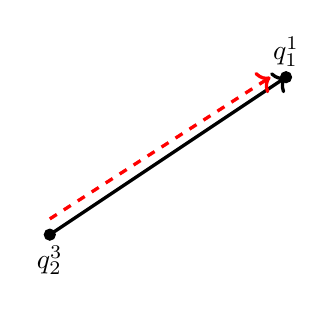
\begin{tikzpicture}
\filldraw[black] (27, 0) circle (2pt);
\filldraw[black] (30, 2) circle (2pt);
\draw[very thick,->] (27, 0)node[anchor=north]{$q_2^3$}  -- (30, 2) node[anchor=south]{$q_1^1$};
\draw[very thick, red, ->, dashed] (27, 0.2) -- (29.8, 2);
\end{tikzpicture}
\end{center}
%
\end{example}
%
%
%

\section{High level Language}
%
\subsection{Syntax and Semantics}
%
\paragraph{Syntax.}
\[
\begin{array}{llll}
 \mbox{Arithmatic Operators} & *_a & ::= & + ~|~ - ~|~ \times 
%
~|~ \div \\  
  \mbox{Boolean Operators} & *_b & & \\
   \mbox{Relational Operators} & *_r & ::= & < ~|~ \leq ~|~ = \\  
 \mbox{Label} & l & & \\ 
 \mbox{While Map} & w & \in & \mbox{Label} \times \mathbb{N} \\
\mbox{AExpr} & \aexpr & ::= & 
	%
	n ~|~ x ~|~ \aexpr *_a \aexpr ~|~ \jl{[] ~|~ [\aexpr_0, \dots, \aexpr_i] ~|~ \uniform ~|~ \bernoulli ~|~ \aexpr \times \aexpr } \\
    %
\mbox{BExpr} & \bexpr & ::= & 
	%
	\etrue ~|~ \efalse  ~|~ \neg \bexpr
	 ~|~ \bexpr *_b \bexpr
	%
	~|~ \aexpr *_r \aexpr \\
\mbox{Command} & c & ::= &   [\assign x \expr]^{l} ~|~  [\assign x q(\expr)]^{l}
%
 \\
	%
& & & ~|~  c ; c ~|~ \eif([\bexpr]^{l}, c_1, c_2) 
	~|~ \ewhile([\bexpr]^{l}, c) ~|~ [\eskip]^{l} \sep \jl{\eloop ~ [\valr_N]^{l} ~ (f) ~ \edo ~ c }
	\\
\mbox{Memory} & m & ::= & [] ~|~ m[x^{l} \to v] \\
%
\mbox{Trace} & t & ::= & [] ~|~ [(q, v)^{(l, w) }] ~|~ t ++ t
\end{array}
\]
%
%
\begin{example}
\textbf{Dependency graphs for high level programs containing  non-atomic queries}
\\
Let $q_1 = \lambda D. D_i * D_j$, \\ 
Let $q_2 (x_1) = \lambda D. D_i * D_j + x_1  $.\\
Let $q_3 (x_1 - x_2) = \lambda D. D_i * D_j + x_1 - x_2 $, 
$q_4 (x_2) = \lambda D. D_i * D_j + x_2 $, 
and $q_5(x_1) = \lambda D. D_i * D_j + x_1$ .\\
in program $P_1$, $P_2$ and $P_3$ as following:
\[
P_1 \triangleq
\begin{array}{c}
      \left[\assign{x_1}{q_1} \right]^1; \\
   \left[\assign{x_2}{q_2} \right]^2 ; \\
     \left[\assign{x_3}{q_3} \right]^3
\end{array}
\hspace{2cm}
P_2 \triangleq
\begin{array}{c}
      \left[\assign{x_1}{q_1} \right]^1; \\
   \left[\assign{x_2}{q_2} \right]^2 ; \\
     \left[\assign{x_3}{q_4} \right]^3
\end{array}
\hspace{2cm}
P_3 \triangleq
\begin{array}{c}
      \left[\assign{x_1}{q_1} \right]^1; \\
   \left[\assign{x_2}{q_2} \right]^2 ; \\
     \left[\assign{x_3}{q_5} \right]^3
\end{array}
\]
%
\begin{center}
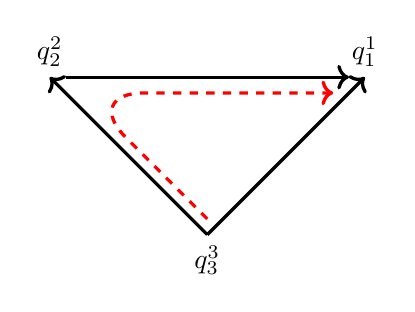
\begin{tikzpicture}
\draw[very thick,->] (8, 0)node[anchor=north]{$q_3^3$} -- (6, 2) node[anchor=south]{$q_2^2$};
\draw[very thick,->] (8, 0)  -- (10, 2) node[anchor=south]{$q_1^1$};
\draw[very thick,->] (6.2, 2) -- (9.8, 2);
%%%%%draw the longest path
\draw[rounded corners=8mm, very thick, red, dashed, ->] (8, 0.2) -- (6.4, 1.8) -- (9.6, 1.8);
\end{tikzpicture}
%
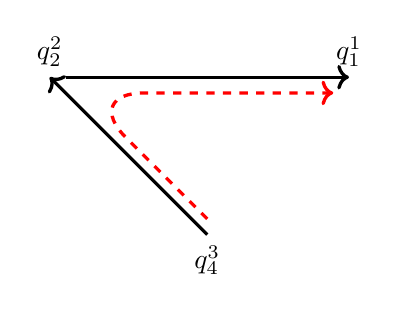
\begin{tikzpicture}
\draw[very thick,->] (18, 0)node[anchor=north]{$q_4^3$} -- (16, 2) node[anchor=south]{$q_2^2$};
\draw[very thick,->] (16.2, 2) -- (19.8, 2)node[anchor=south]{$q_1^1$};
\draw[rounded corners=8mm, very thick, red, dashed, ->] (18, 0.2) -- (16.4, 1.8) -- (19.6, 1.8);
\end{tikzpicture}
%
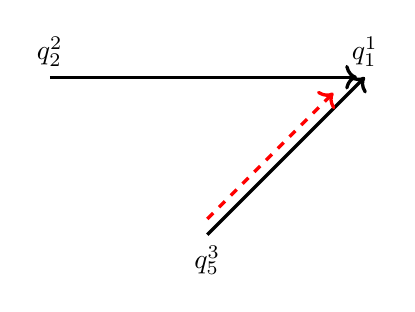
\begin{tikzpicture}
\draw[very thick,->] (26, 2) node[anchor=south]{$q_2^2$} -- (29.9, 2);
\draw[very thick,->] (28, 0)node[anchor=north]{$q_5^3$}  -- (30, 2) node[anchor=south]{$q_1^1$};
% \draw[very thick, red, ->, dashed] (26.4, 1.8) -- (29.6, 1.8);
\draw[very thick, red, ->, dashed] (28, 0.2) -- (29.6, 1.8);
\end{tikzpicture}
\end{center}
%
\end{example}
%
\subsection{Rewriting from High Level Program into Low Level Program}
%
The transformation $\ts{e^h} = e^l$ transfers the expression $e^h$ in the high level language to an expression $e_l$ in the low language. 
Let us look at the special cases: the query.
\\
In the first transition, if a query in high level language isn't atomic, i.e., 
$q(e)$ depends on $e$ with free variables, then it will be rewrite into a switch command. 
This rewriting will switch on the possible values $v_i$ of $e$ and convert the $q(e)$ into a series of atomic queries $q_i$.
\\
In the second transition, if a query in high level language is atomic, $q()$ only depends on data base $D$ and some constant values,
then it will be rewrite into identity in our low level language.
\\
Another special case is the sampling command in high level language. To exclude the dependency caused by the randomness, we will rewrite the sampling into an assignment command in low level language. This will assign a constant value to the corresponding variable.
\\
The resting commands will be rewrote identically.
%
%
\[
\begin{array}{lll}
\ts{ [\assign x q(e)]^{l}}
        & \Rightarrow &
        \left[
        \begin{array}{l}
             \eswitch ~ \Bigg(\expr, x, 
            \left(\begin{array}{l}
           v_1 \to q_1, \\
            \cdots, \\
            v_m \to q_m
            \end{array}\right) 
            \Bigg) \\
        \end{array}
        \right]^{l}\\
    \ts{q()} & \Rightarrow & q\\
  \ts{[\assign{x}{\uniform} ]^{l}}   &   \Rightarrow & \left[
\assign x c_{u}
\right]^{l} \\
 \ts{[\assign{x}{\expr} ]^{l}}   &   \Rightarrow & \left[ \assign x \expr \right]^{l} \\
 \ts{ c_1 ; c_2 }     & \Rightarrow  & \ts{c_1} ; \ts{c_2} \\
  \ts{\eif([\bexpr]^{l}, c_1, c_2)}  &  \Rightarrow & \eif([\bexpr]^{l}, \ts{c_1}, \ts{c_2}) \\
 \ts{\ewhile([\bexpr]^{l}, c)} & \Rightarrow & \ewhile([\bexpr]^{l},  \ts{c} ) \\
\end{array}
\]
%
%
\begin{example}[Two Round Algorithm]
\[
TR^H(k) \triangleq
\ts{
\begin{array}{l}
    \left[j \leftarrow 1 \right]^1 ; \\
    \left[a \leftarrow [] \right]^2; \\
    \ewhile \Big( 
    \left[j \leq k \right]^3 , \\
     \left[x \leftarrow q_j() \right]^4 ; \\
    \left[a \leftarrow x :: a \right]^5;\\
    \left[j \leftarrow j + 1 \right]^6
    \Big);\\
    \clabel{l \leftarrow q_{k + 1}(a)}^7;\\
\end{array}
}
%
~~~~~~~~ \Rightarrow ~~~~~~~
%
TR^L \triangleq
\begin{array}{l}
    \left[j \leftarrow 1 \right]^1 ; \\
    \left[a \leftarrow [] \right]^2; \\
    \ewhile \Big( 
    \left[j \leq k \right]^3, \\
     \left[x \leftarrow q_j \right]^4; \\
    \left[a \leftarrow x :: a \right]^5;\\
    \left[j \leftarrow j + 1 \right]^6
    \Big);\\
    \clabel{
\eswitch \Bigg(a, x, 
    \left(\begin{array}{l}
    \left[-n, -n, -n, \cdots, -n\right] \to q_{k + 1,1},\\
    \cdots\\
    \left[n, n, n, \cdots, n\right] \to q^{}_{k + 1, n^k}
\end{array} \right) \Bigg)
    }^7
\end{array}
\]
$\config{\emptyset, TR^L, D, [],\emptyset} \rightarrow \config{m, \eskip, D, t, w } $.
$$t = [ (q_1^{(4, \{3 \to 1\} )},v_1 ), (q_2^{(4, \{3 \to 2\} )},v_2 ), \ldots, (q_k^{(4, \{3 \to k\} )},v_k ) , (q_{k+1, i }^{(7, \emptyset )},v_1 )  ] $$
%
A($TR^L$) = 1

\begin{center}
%
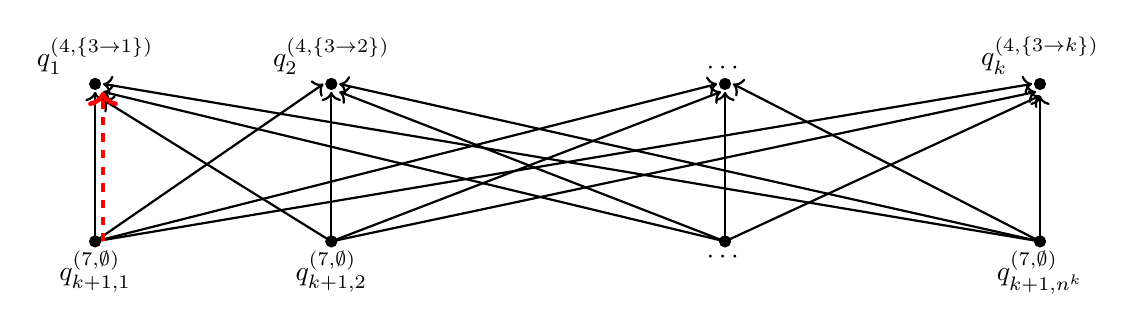
\begin{tikzpicture}
%%% The nodes represents the k query in the first round
\filldraw[black] (0, 2) circle (2pt) node [anchor=south]{$q_1^{(4, \{3 \to 1\} )}$};
\filldraw[black] (3, 2) circle (2pt) node [anchor=south]{$q_2^{(4, \{3 \to 2\} )}$};
% \filldraw[black] (6, 2) circle (2pt) node [anchor=south]{$q^4_3$};
\filldraw[black] (8, 2) circle (2pt) node [anchor=south]{$\cdots$};
\filldraw[black] (12, 2) circle (2pt) node [anchor=south]{$q_k^{(4, \{3 \to k\} )}$};
%%%%%% The nodes represents the n^k queries in the second round
\filldraw[black] (0, 0) circle (2pt) node [anchor=north]{$q_{k+1,1}^{(7, \emptyset)}$};
\filldraw[black] (3, 0) circle (2pt) node [anchor=north]{$q_{k+1,2}^{(7, \emptyset)}$};
% \filldraw[black] (6, 0) circle (2pt) node [anchor=north]{$q^{3, 7}_{k+1}$};
\filldraw[black] (8, 0) circle (2pt) node [anchor=north]{$\cdots$};
\filldraw[black] (12, 0) circle (2pt) node [anchor=north]{$q_{k+1,n^k}^{(7, \emptyset)}$};
%%%%%% The edges represents their dependency relations GROUP 1
\draw[ thick,->] (0, 0)  -- (0, 1.9) ;
\draw[ thick,->] (0, 0)  -- (2.9, 2) ;
% \draw[very thick,->] (0, 0)  -- (6, 2) ;
\draw[ thick,->] (0, 0)  -- (7.9, 2) ;
\draw[ thick,->] (0, 0)  -- (11.9, 2) ;
%%%%%% The edges represents their dependency relations GROUP 2
\draw[ thick,->] (3, 0)  -- (0.1, 1.8) ;
\draw[ thick,->] (3, 0)  -- (3, 1.9) ;
% \draw[very thick,->] (0, 0)  -- (6, 2) ;
\draw[ thick,->] (3, 0)  -- (7.95, 1.9) ;
\draw[ thick,->] (3, 0)  -- (11.95, 1.9) ;
%%%%%% The edges represents their dependency relations GROUP 3
\draw[ thick,->] (8, 0)  -- (0.1, 1.9) ;
\draw[ thick,->] (8, 0)  -- (3.1, 1.9) ;
% \draw[very thick,->] (0, 0)  -- (6, 2) ;
\draw[ thick,->] (8, 0)  -- (8, 1.9) ;
\draw[ thick,->] (8, 0)  -- (12, 1.85) ;
%%%%%% The edges represents their dependency relations GROUP 4
\draw[ thick,->] (12, 0)  -- (0.1, 2) ;
\draw[ thick,->] (12, 0)  -- (3.1, 2) ;
% \draw[very thick,->] (0, 0)  -- (6, 2) ;
\draw[ thick,->] (12, 0)  -- (8.1, 2) ;
\draw[ thick,->] (12, 0)  -- (12, 1.85) ;
%%%% The longest path representing the adaptivity
\draw[ultra thick, red, ->, dashed] (0.1, 0) -- (0.1, 1.9);
\end{tikzpicture}
\end{center}
\end{example}
%
%
\begin{example}[Multi-Round Algorithm]
\[
MR^H \triangleq
\begin{array}{l}
     \left[j \leftarrow 0 \right]^1 ; \\
    \left[I \leftarrow [] \right]^2; \\
    \ewhile \Big( 
    \left[j \leq k \right]^3 , \\
    \left[p \leftarrow \uniform(0,1) \right]^4 ; \\
    \left[a \leftarrow q_j(p, I) \right]^5; \\
    \left[I \leftarrow \eupdt(I, (a, p))  \right]^6;\\
    \left[j \leftarrow j + 1 \right]^7
    \Big) ;
\end{array}
%
~~~~ \Rightarrow ~~~
%
MR^L \triangleq
\begin{array}{l}
     \left[j \leftarrow 0 \right]^1 ; \\
    \left[I \leftarrow [] \right]^2; \\
    \ewhile \Big( 
    \left[j \leq k \right]^3 , \\
    \left[p \leftarrow 0 \right]^4 ; \\
    \left[
    \eswitch \Big( I, x
    \left(\begin{array}{l}
        [ ] \to q_{j,1},\\
        \cdots\\
    \clabel{1, 2, 3, \cdots, n} \to q_{j,n!}
    \end{array}\right)
    \Big)
    \right]^5\\
    \clabel{I \leftarrow \eupdt(I, (a, p))}^6;\\
    \clabel{j \leftarrow j + 1 }^7
    \Big) ;
\end{array}
\]
%
%
Let $k = 4$, given a specific database $D$, we have $\config{\emptyset, MR^L, D, [],\emptyset} \rightarrow \config{m, \eskip, D, t, w } $ and the trace as:
%
$$t = \left[(q^{5, \{3 \to 1\}}_{1, 1}, v_1), 
(q^{5, \{3 \to 2\}}_{2, 3}, v_2),
(q^{5, \{3 \to 3\}}_{3, 2}, v_3)
(q^{5, \{3 \to 4\}}_{4, 3}, v_4)
\right]$$
\\
A($TR^L$) = 3
\begin{center}
%
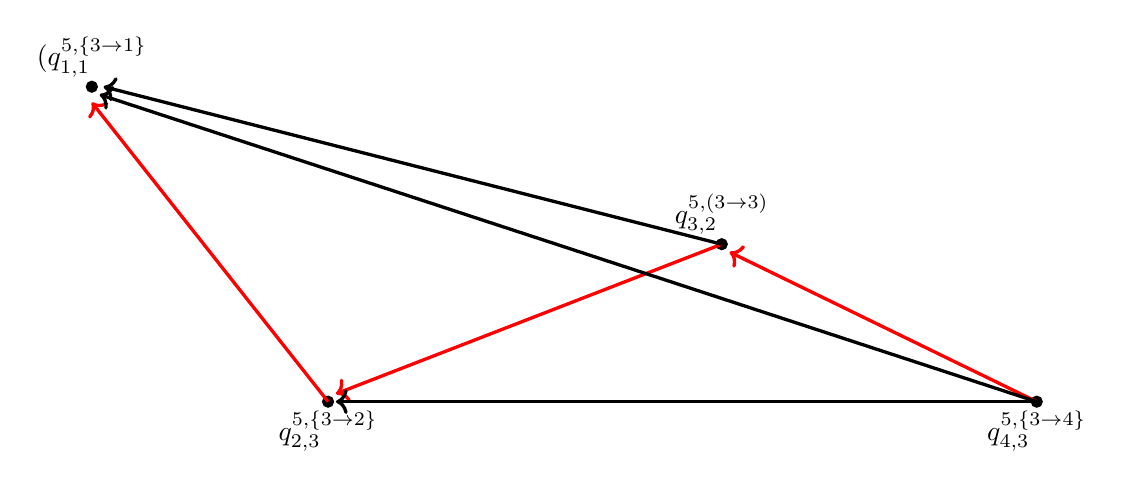
\begin{tikzpicture}
%%% The nodes represents the k query in the first round
\filldraw[black] (0, 4) circle (2pt) node [anchor=south]{$(q^{5, \{3 \to 1\}}_{1, 1}$};
% \filldraw[black] (8, 4) circle (2pt) node [anchor=south]{$\cdots$};
% \filldraw[black] (12, 4) circle (2pt) node [anchor=south]{$q^{1, (5, k)}_k$};
%%%%%% The nodes represents the n^k queries in the second round
% \filldraw[black] (0, 0) circle (2pt) node [anchor=north]{$q^{n!, (5, 1)}_1$};
\filldraw[black] (3, 0) circle (2pt) node [anchor=north]{$q^{5, \{3 \to 2\}}_{2, 3}$};
% \filldraw[black] (6, 0) circle (2pt) node [anchor=north]{$q^{3, 7}_{k+1}$};
% \filldraw[black] (8, 0) circle (2pt) node [anchor=north]{$\cdots$};
\filldraw[black] (12, 0) circle (2pt) node [anchor=north]{$q^{5, \{3 \to 4\}}_{4, 3}$};
%%% The nodes represents the k query in the first round
% \filldraw[black] (0, 2) circle (2pt) node [anchor=south]{$q^{\cdots, (5, 1)}_1$};
% \filldraw[black] (3, 2) circle (2pt) node [anchor=south]{$q^{\cdots, (5, 2)}_2$};
% \filldraw[black] (6, 2) circle (2pt) node [anchor=south]{$q^4_3$};
\filldraw[black] (8, 2) circle (2pt) node [anchor=south]{$q^{5, (3 \to 3)}_{3, 2}$};
% \filldraw[black] (12, 2) circle (2pt) node [anchor=south]{$q^{\cdots, (5, k)}_k$};
%%%%%% The edges represents their dependency relations GROUP 1
% \draw[very thick,->] (3, 2)  -- (0.1, 2) ;
% \draw[very thick,->] (3, 0)  -- (0.1, 1.9) ;
% \draw[very thick,->] (3, 4)  -- (0.1, 2.1) ;
% %
% \draw[very thick,->] (3, 2)  -- (0.1, 0.1) ;
% \draw[very thick,->] (3, 0)  -- (0.1, 0) ;
% \draw[very thick,->] (3, 4)  -- (0, 0.2) ;
% %
% \draw[very thick,->] (3, 2)  -- (0.1, 3.9) ;
\draw[very thick,->, red] (3, 0)  -- (0, 3.8) ;
% \draw[very thick,->] (3, 4)  -- (0, 4) ;
% \draw[very thick,->] (0, 0)  -- (6, 2) ;
%%%%%% The edges represents their dependency relations GROUP 2
% \draw[very thick,->] (0, 0)  -- (6, 2) ;
% \draw[very thick,->] (8, 2)  -- (3.1, 2) ;
% \draw[very thick,->] (8, 0)  -- (3.1, 1.9) ;
% \draw[very thick,->] (8, 4)  -- (3.1, 2.1) ;
%
\draw[very thick,->, red] (8, 2)  -- (3.1, 0.1) ;
\draw[very thick,->] (8, 2)  -- (0.15, 4) ;
% \draw[very thick,->] (8, 0)  -- (3.1, 0) ;
% \draw[very thick,->] (8, 4)  -- (3, 0.2) ;
% %
% \draw[very thick,->] (8, 2)  -- (3.1, 3.9) ;
% \draw[very thick,->] (8, 0)  -- (3, 3.8) ;
% \draw[very thick,->] (8, 4)  -- (3.1, 4) ;
%%%%%% The edges represents their dependency relations GROUP 4
% \draw[very thick,->] (0, 0)  -- (6, 2) ;
% \draw[very thick,->] (12, 2)  -- (8.1, 2) ;
\draw[very thick,->, red] (12, 0)  -- (8.1, 1.9) ;
\draw[very thick,->] (12, 0)  -- (3.1, 0) ;
\draw[very thick,->] (12, 0)  -- (0.1, 3.9) ;
% \draw[very thick,->] (12, 4)  -- (8.1, 2.1) ;
% %
% \draw[very thick,->] (12, 2)  -- (8.1, 0.1) ;
% \draw[very thick,->] (12, 0)  -- (8.1, 0) ;
% \draw[very thick,->] (12, 4)  -- (8, 0.2) ;
% %
% \draw[very thick,->] (12, 2)  -- (8.1, 3.9) ;
% \draw[very thick,->] (12, 0)  -- (8, 3.8) ;
% \draw[very thick,->] (12, 4)  -- (8.1, 4) ;
%
% \draw[very thick,->] (12, 2)  -- (8.1, 3.9) ;

%%%% The longest path representing the adaptivity
% \draw[ultra thick, red, ->, dashed] (3, 4.1)  -- (0.1, 4.1);
% \draw[ultra thick, red, ->, dashed] (8, 4.1)  -- (3.1, 4.1);
% \draw[ultra thick, red, ->, dashed] (12, 4.1)  -- (8.1, 4.1);
\end{tikzpicture}
\end{center}
%
%
$\forall k. \forall D$, we have $A(TR^L) = (k - 1)$ given all possible execution traces.
\begin{center}
%
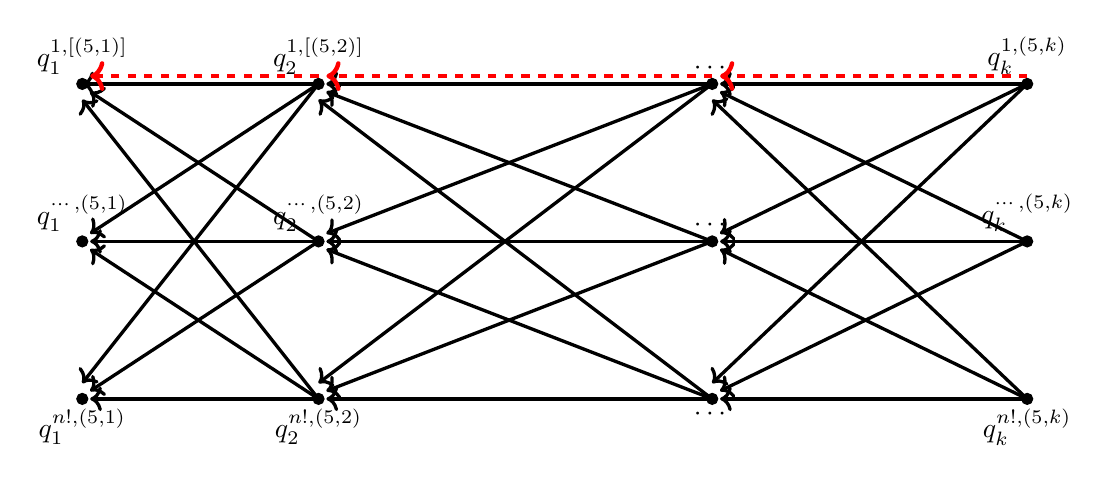
\begin{tikzpicture}
%%% The nodes represents the k query in the first round
\filldraw[black] (0, 4) circle (2pt) node [anchor=south]{$q^{1, [(5, 1)]}_1$};
\filldraw[black] (3, 4) circle (2pt) node [anchor=south]{$q^{1, [(5, 2)]}_2$};
% \filldraw[black] (6, 2) circle (2pt) node [anchor=south]{$q^4_3$};
\filldraw[black] (8, 4) circle (2pt) node [anchor=south]{$\cdots$};
\filldraw[black] (12, 4) circle (2pt) node [anchor=south]{$q^{1, (5, k)}_k$};
%%%%%% The nodes represents the n^k queries in the second round
\filldraw[black] (0, 0) circle (2pt) node [anchor=north]{$q^{n!, (5, 1)}_1$};
\filldraw[black] (3, 0) circle (2pt) node [anchor=north]{$q^{n!, (5, 2)}_2$};
% \filldraw[black] (6, 0) circle (2pt) node [anchor=north]{$q^{3, 7}_{k+1}$};
\filldraw[black] (8, 0) circle (2pt) node [anchor=north]{$\cdots$};
\filldraw[black] (12, 0) circle (2pt) node [anchor=north]{$q^{n!, (5, k)}_k$};
%%% The nodes represents the k query in the first round
\filldraw[black] (0, 2) circle (2pt) node [anchor=south]{$q^{\cdots, (5, 1)}_1$};
\filldraw[black] (3, 2) circle (2pt) node [anchor=south]{$q^{\cdots, (5, 2)}_2$};
% \filldraw[black] (6, 2) circle (2pt) node [anchor=south]{$q^4_3$};
\filldraw[black] (8, 2) circle (2pt) node [anchor=south]{$\cdots$};
\filldraw[black] (12, 2) circle (2pt) node [anchor=south]{$q^{\cdots, (5, k)}_k$};
%%%%%% The edges represents their dependency relations GROUP 1
\draw[very thick,->] (3, 2)  -- (0.1, 2) ;
\draw[very thick,->] (3, 0)  -- (0.1, 1.9) ;
\draw[very thick,->] (3, 4)  -- (0.1, 2.1) ;
%
\draw[very thick,->] (3, 2)  -- (0.1, 0.1) ;
\draw[very thick,->] (3, 0)  -- (0.1, 0) ;
\draw[very thick,->] (3, 4)  -- (0, 0.2) ;
%
\draw[very thick,->] (3, 2)  -- (0.1, 3.9) ;
\draw[very thick,->] (3, 0)  -- (0, 3.8) ;
\draw[very thick,->] (3, 4)  -- (0, 4) ;
% \draw[very thick,->] (0, 0)  -- (6, 2) ;
%%%%%% The edges represents their dependency relations GROUP 2
% \draw[very thick,->] (0, 0)  -- (6, 2) ;
\draw[very thick,->] (8, 2)  -- (3.1, 2) ;
\draw[very thick,->] (8, 0)  -- (3.1, 1.9) ;
\draw[very thick,->] (8, 4)  -- (3.1, 2.1) ;
%
\draw[very thick,->] (8, 2)  -- (3.1, 0.1) ;
\draw[very thick,->] (8, 0)  -- (3.1, 0) ;
\draw[very thick,->] (8, 4)  -- (3, 0.2) ;
%
\draw[very thick,->] (8, 2)  -- (3.1, 3.9) ;
\draw[very thick,->] (8, 0)  -- (3, 3.8) ;
\draw[very thick,->] (8, 4)  -- (3.1, 4) ;
%%%%%% The edges represents their dependency relations GROUP 4
% \draw[very thick,->] (0, 0)  -- (6, 2) ;
\draw[very thick,->] (12, 2)  -- (8.1, 2) ;
\draw[very thick,->] (12, 0)  -- (8.1, 1.9) ;
\draw[very thick,->] (12, 4)  -- (8.1, 2.1) ;
%
\draw[very thick,->] (12, 2)  -- (8.1, 0.1) ;
\draw[very thick,->] (12, 0)  -- (8.1, 0) ;
\draw[very thick,->] (12, 4)  -- (8, 0.2) ;
%
\draw[very thick,->] (12, 2)  -- (8.1, 3.9) ;
\draw[very thick,->] (12, 0)  -- (8, 3.8) ;
\draw[very thick,->] (12, 4)  -- (8.1, 4) ;
%
%%%% The longest path representing the adaptivity
\draw[ultra thick, red, ->, dashed] (3, 4.1)  -- (0.1, 4.1);
\draw[ultra thick, red, ->, dashed] (8, 4.1)  -- (3.1, 4.1);
\draw[ultra thick, red, ->, dashed] (12, 4.1)  -- (8.1, 4.1);
\end{tikzpicture}
\end{center}
\end{example}
%
%
\clearpage
\section{Towards Probability}
%
\subsection{Syntax and Semantics}
%
\paragraph{Syntax.}
\[
\begin{array}{llll}
 \mbox{Arithmatic Operators} & *_a & ::= & + ~|~ - ~|~ \times 
%
~|~ \div \\  
  \mbox{Boolean Operators} & *_b & ::= & \lor \sep \land \\
   \mbox{Relational Operators} & *_r & ::= & < ~|~ \leq ~|~ = \\  
 \mbox{Label} & l & & \\ 
 \mbox{While Map} & w & \in & \mbox{Label} \times \mathbb{N} \triangleq w +l \sep w \setminus l \sep w \oplus_\rho w \\
\mbox{AExpr} & \aexpr & ::= & 
	%
	n ~|~ x ~|~ \aexpr *_a \aexpr ~|~ {[] ~|~ [\aexpr_0, \dots, \aexpr_i] \sep \aexpr \times \aexpr } \\
    %
\mbox{BExpr} & \bexpr & ::= & 
	%
	\etrue ~|~ \efalse  ~|~ \neg \bexpr
	 ~|~ \bexpr *_b \bexpr
	%
	~|~ \aexpr *_r \aexpr \\
\mbox{Deterministic Expr} & \expr_d & ::=	& \aexpr \sep \bexpr \\
\mbox{Randomized AExpr} & \aexpr_r & ::= & 
	%
	 x_r \sep n \sep  \aexpr_r *_a \aexpr_r \\
    %
\mbox{Randomized BExpr} & \bexpr_r & ::= & 
	%
\neg \bexpr_r
	 ~|~ \bexpr_r *_b \bexpr_r
	%
	~|~ \aexpr_r *_r \aexpr_r \\
\mbox{Randomized Expr} & \expr_r & ::=	& \expr_d \sep \aexpr_r \sep \bexpr_r \\
\mbox{Command} & C & ::= &   [\assign x {\expr_d}]^{l} \sep [\assign {x_r} {\expr_r}]^{l} \sep  [\assign x q]^{l} \sep  [\assign {x_r} \uniform ]^{l} \sep   [\assign {x_r} \bernoulli]^{l} 
 %
\\
	%
& & & ~|~  \command ; \command  ~|~ \eif_D ([\bexpr]^{l}, \command_1, \command_2) \sep  \eif_R ([\bexpr_r]^{l}, \command_1, \command_2) 
	~|~ \ewhile([\bexpr]^{l}, \command) ~|~ [\eskip]^{l} \\
& & &	~|~ {\eunfold{[\bexpr]^{l}}{\command} \sep [\eswitch( \expr, x, (v_i \to  q_i))]^{l}} \sep \jl{\eloop ~ [\valr_N]^{l} ~ (f) ~ \edo ~ \command }
	\\
	%
% \mbox{Binary Operation} & \bop & ::= & + ~|~ - ~|~ \times 
% %
\mbox{Memory} & m & ::= & [] ~|~ m[x^{l} \to v] \\
%
\mbox{Trace} & t & ::= & [] ~|~ [(q, v)^{(l, w) }] ~|~ t ++ t 
~|~ t \oplus_{\rho} t
\end{array}
\]
%
\[
\begin{array}{ccl}
w \setminus l     & = &\left \{  
    \begin{array}{lr} w  & l \not\in Keys(w)   \\
      w_l & Otherwise \\
     \end{array} \right.\\
w + l & = &
 \left \{  
    \begin{array}{lr}
    w[l \to 0] & l \not \in Keys(w) \\   
    w_l [l \to w(l)+1] & Otherwise
          \end{array} \right.\\
\end{array}
\]
%
\paragraph{Semantics}
We have a countable set $\textsf{RV}$ of random variables($x_r \in \textsf{RV}$), a countable set $\textsf{Val}$ of values. For any subset  $\textsf{S} \subseteq \textsf{RV}$, we denote $\textsf{RanM[S]} \triangleq \textsf{S} \to \textsf{Val} $. We let $\textsf{DV}$ as a countable set of deterministic variables ($x$) and the deterministic memory $\textsf{DetM} \triangleq \textsf{DV} \to \textsf{Val}$. 
Distribution over A as $D(A)$. The \emph{distribution unit} unit : $A \to D(A)$. The \emph{distribution bind} bind : $ D(A) \to (A \to D(B)) \to D(B)$. $\lrr{C}{} : (\textsf{DetM} \times D(\textsf{RandM}) \times \textsf{Trace} \times \textsf{WhileMap} \times \textsf{DB} ) \to (\textsf{DetM} \times D(\textsf{RandM}) \times \textsf{Trace} \times \textsf{WhileMap} \times \textsf{DB} ) $

\[\config{(\sigma, \mu_1 , t_1, w_1, D)} \oplus_{\rho} \config{(\sigma, \mu_2 , t_2, w_2, D)} 
\triangleq \config{\sigma, \mu_1\oplus_{\rho} \mu_2 , t_1\oplus_{\rho} t_2, w_1 \oplus_{\rho} w_2, D}\]
%
\[(t_1 \oplus_{\rho} t_2)  ++ t_3 \triangleq 
(t_1 ++ t_3) \oplus_{\rho} (t_2 ++ t_3) \]
%
\[t_3 ++ (t_1 \oplus_{\rho} t_2) \triangleq 
(t_3 ++ t_1) \oplus_{\rho} (t_3 ++ t_2) \]
%
\[ (w_1 \oplus_{\rho} w_2) + l \triangleq 
(w_1 + l) \oplus_{\rho} (w_2 + l) \]
%
\[ (w_1 \oplus_{\rho} w_2) \setminus l \triangleq 
(w_1 \setminus l) \oplus_{\rho} (w_2 \setminus l) \]
\begin{figure}[H]%
    \centering
    \[
    \begin{array}{rll}
        \lrr{ [\eskip]^{l} }{} (\sigma, \mu , t, w, D) & \triangleq & (\sigma, \mu , t, w , D)  \\
        \lrr{ [\assign x {\expr_d}]^{l} }{} (\sigma, \mu , t, w, D)  & \triangleq & (\sigma[x \to \lrr{\expr_d}{}(\sigma)], \mu , t, w, D) \\
        \lrr{ [\assign {x_r} {\expr_r}]^{l}}{} (\sigma, \mu , t, w, D)  & \triangleq & (\sigma, bind(\mu , m \to unit(m[x_r \to \lrr{\expr_r}{}(\sigma, m)]) ) , t, w , D ) \\
        \lrr{ [\assign x q]^{l} }{} (\sigma, \mu , t, w, D)  & \triangleq & (\sigma[x \to v ], \mu , t ++ [(q, v)]^{(l, w)}, w , D) \qquad : v = q(D)\\
        \lrr{ [\assign {x_r} \uniform ]^{l} }{} (\sigma, \mu , t, w, D)  & \triangleq & (\sigma,  bind(\mu , m \to bind(\uniform , u \to m[x_r \to u] ) )  , t, w, D) \\
        \lrr{ [\assign {x_r} \bernoulli ]^{l} }{} (\sigma, \mu , t, w , D)  & \triangleq & (\sigma , bind(\mu , m \to bind(\bernoulli , u \to m[x_r \to u] ) ) , t, w,D) \\
            \lrr{ \command ; \command' }{} (\sigma, \mu , t, w , D)  & \triangleq & \lrr{\command'}{} ( \lrr{\command}{} \sigma , \mu, t, w) \\
         \lrr{ \eif_D ([\bexpr]^{l}, \command_1, \command_2)  }{} (\sigma, \mu , t, w , D)  & \triangleq & \left \{  \begin{array}{l} 
         \lrr{\command_1}{} (\sigma , \mu, t, w, D) \qquad : \lrr{\bexpr}{}(\sigma) = \etrue \\ 
         \lrr{\command_1}{} (\sigma , \mu, t, w,D) \qquad : \lrr{\bexpr}{}(\sigma) = \efalse \end{array} \right . \\    
           \lrr{ \eif_R ([\bexpr_r]^{l}, \command_1, \command_2)  }{} (\sigma, \mu , t, w , D)  & \triangleq & \left \{
           \begin{array}{l}
           \lrr{\command_1}{} (\sigma , \mu | \lrr{\bexpr_r}{} \sigma = \etrue  , t, w, D) \oplus_\rho  \lrr{\command_2}{} (\rho , \mu | \lrr{\bexpr_r}{} \sigma = \efalse  , t, w,D)  \\ 
           \lrr{\command_1}{} (\sigma , \mu | \lrr{\bexpr_r}{} \sigma = \etrue  , t, w, D) \qquad \rho = 1 \\
           \lrr{\command_2}{} (\sigma , \mu | \lrr{\bexpr_r}{} \sigma = \efalse  , t, w,D) \qquad \rho = 0 \\
            \end{array} \right . \\
             & & \textsf{where} \quad \rho = \mu (\lrr{\bexpr_r}{} \sigma = \etrue ) \\
          \lrr{ \ewhile([\bexpr]^{l}, \command) }{} (\sigma, \mu , t, w , D)  & \triangleq & \lrr{\eunfold{[\bexpr]^{l}}{ \ewhile([\bexpr]^{l}, \command) }   }{} (\sigma, \mu , t, w , D) \\
           \lrr{ \eunfold{[\bexpr]^{l}}{\command}  }{} (\sigma, \mu , t, w , D)  & \triangleq & \left \{  \begin{array}{l} \lrr{\command}{} (\sigma , \mu, t, w + l, D) \qquad : \lrr{\bexpr}{}(\sigma) = \etrue \\ \lrr{\eskip}{} (\sigma , \mu, t, w-l, D) \qquad : \lrr{\bexpr}{}(\sigma) = \efalse \end{array} \right . \\  
           \lrr{ {[\eswitch( \expr, x, (v_i \to  q_i))]^{l}} }{} (\sigma, \mu , t, w , D)  & \triangleq & 
          \lrr{ [\assign x q_1]^{l} }{} ( \sigma, \mu , t, w, D ) 
          \qquad : v_1 = \lrr{\expr}{}{(\sigma)} \\ 
           \lrr{ \jl{\eloop ~ [\expr_N]^{l} ~ (f) ~ \edo ~ \command } }{} (\sigma, \mu , t, w , D)  & \triangleq & \left \{  \begin{array}{l} \lrr{f;\command; \eloop ~ [\expr_N-1]^{l} ~ (f) ~ \edo ~ \command }{} (\sigma , \mu, t, w + l, D) \qquad : \lrr{\expr_N}{}(\sigma) >0 \\ \lrr{\eskip}{} (\sigma , \mu, t, w-l, D) \qquad : \lrr{\expr_N}{}(\sigma) = 0 \end{array} \right . \\  
    \end{array}
    \]
    \caption{Semantics of programs}
    \label{fig:my_label}
\end{figure}
%
%
\[
\begin{array}{l}
     \left[j \leftarrow 0 \right]^1 ; \\
    \left[I \leftarrow [] \right]^2; \\
    \ewhile \Big( 
    \left[j \leq k \right]^3 , \\
    \left[p \leftarrow 0 \right]^4 ; \\
    \left[
    \eswitch \Big( I, x
    \left(\begin{array}{l}
        [ ] \to q_{j,1},\\
        \cdots\\
    \clabel{1, 2, 3, \cdots, n} \to q_{j,n!}
    \end{array}\right)
    \Big)
    \right]^5\\
    \clabel{I \leftarrow \eupdt(I, (x, p))}^6;\\
    \clabel{j \leftarrow j + 1 }^7
    \Big) ;
\end{array}
%
~~~~ \Rightarrow ~~~
%
SSA \triangleq
\begin{array}{l}
     \left[j \leftarrow 0 \right]^1 ; \\
    \left[I_1 \leftarrow [] \right]^2; \\
    \ewhile \Big( 
    \left[j \leq k \right]^3 , \phi: {I_2} = f({I_1}, {I_3}) \\
    \left[p \leftarrow 0 \right]^4 ; \\
    \left[
    \eswitch \Big( {I_2}, x
    \left(\begin{array}{l}
        [ ] \to q_{j,1},\\
        \cdots\\
    \clabel{1, 2, 3, \cdots, n} \to q_{j,n!}
    \end{array}\right)
    \Big)
    \right]^5\\
    \clabel{{I_3} \leftarrow \eupdt({I_2}, (x, p))}^6;\\
    \clabel{j \leftarrow j + 1 }^7
    \Big) ;
\end{array}
\]
%
%
\subsection{Extending Adaptivity onto Probabilistic Program}
%
\begin{defn}
Dependency Forest.
\\
Given a program $P$, a database $D$, 
dependency forest $F(P, D) \triangleq \{ G_1, G_2, \cdots, G_m \}$,
$G_k = (V_k, E_k)$ is defined as: 
\\
$V_k =\{q^{l,w} |\forall m, w. \config{\emptyset, P, D,[], \emptyset } \rightarrow \config{m, \eskip, D, T, \emptyset} \land q^{l,w} \in \pi_k (T)  \}$;
\\
$E_k = \left\{(q_i^{l,w},q_j^{l',w'}) 
~ \left \vert ~ \neg \mathsf{IND}(q_i^{l,w},q_j^{l',w'}, P)
\land \mathsf{To}(q_j^{l',w'}, q_i^{l,w}) \right.\right\}$,
\\
where $\pi_k (T) = t_k$ s.t. $T = t_1 \oplus_{\rho_1} t_2 \oplus_{\rho_2}
\cdots \oplus_{m - 1} t_m $ and there is no $\oplus$ in $t_i$.
\end{defn}

\begin{defn}
Dependency Graph.
\\
Given a program $P$, a database $D$, 
dependency graph $G(P, D) \triangleq (V, E)$ is defined as: 
\\
$V =\bigcup \{V_k | G_k \in F(P, D)  \}$;
\\
$E_k = \left\{(q_i,q_j) 
~ \left \vert ~ (q_i,q_j) \in E_k , G_k \in F(P, D) \right.\right\}$,
\end{defn}
%
%
\begin{defn}
Adaptivity.
\\
Given a program $P$ and for all the database $D$ in a set of $DBS$ of databases, the total dependency graph G is the combination of all the dependent graphs over every single database $G(P, D) = (V, E)$, the adaptivity of the program is defined as $A(P)$, s.t.:
for every pair $(i,j)$ let $p_{(i,j)}$ be the longest path starting from $q_i^{l, w}$ to $q_j^{l',w'}$,
%
$$A(P) = \max\limits_{q_i^{l,w},q_j^{l',w'} \in V }\{l_i ~|~ l_i = |p_(i,j)| \}$$
\end{defn}
%
%
\section{Analysis of Program Adaptivity}
We have the judgment of the form : $\vdash^{c_1, c_2}_{M,V} ~ P : \Phi \implies \Psi$.  Our grade is a combination of a matrix $M$, used to track the dependency of variables appeared in the statement $S$, and a vector $V$ indicating the variables associated with results from queries $q$. The size of the matrix $M$ is $L \times L$, and vector $V$ of size $N$, where $L$ is the total size of variables needed in the program, which is fixed per program. 
The superscript $c_1,c_2$ is a counter specifying the range of "living" or "active" variables in the matrix and vector. $c_1$ is the starting line (and column) in the matrix where the new generated variables  in program $P$ starts to show up. Likewise, $c_2$ states the ending position of active range by $P$. The new generated variables will be treated carefully when we handle recursive statement, in our case, the loop statement. 

We assume the program $P$ is in the static single assignment form. That is to say, $x \leftarrow e_1; x \leftarrow e_2 $ will be rewritten as $ x_1 \leftarrow e_1; x_2 \leftarrow e_2$. And the if condition $ \eif ~ e_b \ethen x \leftarrow e_1 \eelse x \leftarrow e_2  $ will look like $ \eif ~ e_b \ethen x_1 \leftarrow e_1 \eelse x_2 \leftarrow e_2  $. As we have seen, ssa provides unique variables, and these newly generated variables will be recorded in the matrix $M$. Worth to mention, $c_1,c_2$ can be used to track the exact location of newly generated variables. For example, the assignment statement $x \leftarrow e$ or $x \leftarrow q $ holds $c_2 =c_1+1$, telling us the variable $x$ is at the $c_1$th line(column) of the matrix. As we can notice, the loop increases the matrix by $N \times a$ where $N$ is the number of rounds of the loop and $a$ is the size of the variables generated in the loop body $P$.

We will have a global map, which maps the variable name to the position in the vector. We call it $G: VAR \to \mathbb{N}$,

We give an example of $M$ and $V$ of the program $P$. 
$$
P= \begin{array}{c}
\assign {x_1} {q} ;        \\
\assign {x_2} {x_1+1} ;\\
\assign {x_3} {x_2+2} 
\end{array}~~~~~~~~~~~~
M =  \begin{matrix}
 0 & 0 & 0 \\
1 & 0 & 0 \\
1 & 1 & 0 \\
\end{matrix} ~ , V = \begin{matrix}
  1 \\
 0 \\
 0 \\
\end{matrix}
$$


\paragraph{Analysis Rules.}
%
%
\framebox{$ {\Gamma} \vdash^{c_1, c_2}_{M,V} ~ P : \Phi \implies \Psi$}
%
\begin{mathpar}
\inferrule
{M = L(x) * ( R(\expr) + \Gamma )
}
{\Gamma \vdash_{M, V_{\emptyset}}^{(c, c+1)} \assign x \expr :
\Phi \implies \Psi
}
\and
\inferrule
{M = L(x) * ( R(\emptyset) + \Gamma)
\\
V= L(x)
}
{ \Gamma \vdash^{(c, c+1)}_{M, V} \assign x q : 
\Phi \implies \Psi
}
%
\and 
%
\inferrule
{
\Gamma + R(e_b) \vdash^{(c_1, c_2)}_{M_1, V_1} P_1 : 
\Phi \implies \Psi
\and 
\Gamma + R(e_b) \vdash^{(c_2, c_3)}_{M_2, V_2} P_2 :
\Phi \implies \Psi
}
{
\Gamma \vdash^{(c_1, c_3)}_{M_1 \uplus M_2, V_1 \uplus V_2} 
\eif ~ e_b \ethen P_1 \eelse P_2 :\Phi \implies \Psi
}
%
\and 
%
\inferrule
{
\Gamma \vdash^{(c_1, c_2)}_{M_1, V_1} P_1 : \Phi \implies \Psi' \and 
\Gamma \vdash^{(c_2, c_3)}_{M_2, V_2} P_2 : \Psi' \implies \Psi
}
{
\Gamma \vdash^{(c_1, c_3)}_{M_1 \cdot M_2, V_1 \uplus V_2}
P_1 ; P_2
:\Phi \implies \Psi
}
\and 
\inferrule
{
\forall 0 \leq z < N. \Gamma \vdash^{(c, c+a )}_{M, V} f;P : 
\{ \Phi \land \expr_N = z + 1 \} \implies
\{ \Phi \land \expr_N = z \}
}
{\Gamma \vdash^{(c, c+ N*a)}_{M_{c,a}^N(f), V_{c, a}^N} 
\eloop ~ \expr_N ~ (f) ~ \edo ~ P:
\{\Phi \land \expr_N = N\} \implies \{
\Phi \land \expr_N = 0\}
}
%
\and
\inferrule
{ \Gamma + R(\expr) \vdash^{(c_1, c_1+1)}_{M_i, V_i} \assign{ x_i}{q_i} 
\\
i \in \{1, \dots, N\}     }
{\Gamma \vdash^{(c_1, c_1+N)}_{ \sum_{i=0}^{N} M_i, \sum_{i=0}^{N} V_i} \eswitch(\expr, x,(v_i \rightarrow q_i ) }
\end{mathpar}
%
\[
\begin{array}{lll}
V_1 \uplus V_2 & := & \left\{
\begin{array}{ll}
1 & (V_1[i] = 1 \lor V_2[i] = 1) \land i = 1, \cdots, N \land |V_1| = |V_2|\\
0 & o.w.
\end{array}\right.\\
%
M_1 \uplus M_2 & := & \left\{
\begin{array}{ll}
1 & (M_1[i][j] = 1  \lor M_2[i][j] = 1) \land i, j = 1, \cdots, N \land |M_1| = |M_2|\\
0 & (M_1[i][j] = 0  \land M_2[i, j] = 0) \land i, j = 1, \cdots, N \land |M_1| = |M_2|\\
\bot & o.w.
\end{array}\right.\\
%
V_{(c, a)}^N
& := & \left\{
\begin{array}{ll}
V[c+ i*a, c + (i + 1) * a-1] = V[c, c + a-1] & 
 i = 1, \cdots, N - 1 \\
\bot & o.w.
\end{array}\right.\\
%
M_{(c, a)}^N (f)
& := & \left\{
\begin{array}{ll}
M[c+ i*a, c + (i + 1) * a-1][c+ i*a, c + (i + 1) * a-1] & \\
= M[c, c + a-1][c, c+ a-1] & 
 i = 1, \cdots, N - 1 \\
M[c+ i*a, c + (i + 1) * a-1][0, c + (i) * a-1] = 
0 & 
 i = 1, \cdots, N - 1 \\
M[0, c + i * a-1][c+ i*a, c + (i + 1) * a-1] & \\
=  M[0, c + (i - 1) * a-1][c+ (i - 1)*a, c + (i) * a-1] & 
 i = 1, \cdots, N - 1 \\
M[l][k] = 
1& 
\begin{array}{l}
l \in [c + (i - 1)*a, c + (i) *a-1], \\
k \in [c+ i*a, c + (i + 1) * a-1] \\
\land i = 1, \cdots, N 
\land, l= G(x_l) \\
\land k=G(x_k) \land  x_l = f(\cdots, x_k, \cdots)
\end{array}\\
\bot & o.w.
\end{array}\right.\\
%
\end{array}
\]
%
\begin{center}
\begin{tabular}{p{15pt}|p{15pt}|p{15pt}||p{15pt}|p{15pt}
|p{15pt}||p{15pt}|p{15pt}|
p{15pt}|p{15pt}|p{15pt}|p{15pt}|p{15pt}| } 
 1 & $\cdots$ & c-1 & c & $\cdots$ & \tiny{c+a-1} & {\tiny c+a } 
& $\cdots$ & {\tiny{c+2a-1} }
& $\cdots$ & {\tiny c+N*a-1} & {\tiny c+N*a} & $\cdots$ \\
\hline
$\cdots$  & \cellcolor{green} & \cellcolor{green} & \cellcolor{sandstorm} 0 & \cellcolor{sandstorm} 0 & \cellcolor{sandstorm} 0 & \cellcolor{sandstorm} 0 & \cellcolor{sandstorm} 0 & \cellcolor{sandstorm} 0 &  &  &  & \\[10pt]
\hline
c-1 & \cellcolor{green} & \cellcolor{green} & \cellcolor{sandstorm} 0 & \cellcolor{sandstorm} 0 & \cellcolor{sandstorm} 0 & \cellcolor{sandstorm} 0 &\cellcolor{sandstorm} 0 & \cellcolor{sandstorm} 0 &  &  &  &  \\ [10pt]
\hline
c & \cellcolor{periwinkle} & \cellcolor{periwinkle} & \cellcolor{pink} & \cellcolor{pink} &\cellcolor{pink} & \cellcolor{sandstorm} 0 &
\cellcolor{sandstorm} 0 &
\cellcolor{sandstorm} 0 &&&& \\ [10pt]
\hline
$\cdots$ & \cellcolor{periwinkle} & \cellcolor{periwinkle}
&\cellcolor{pink} &\cellcolor{pink}&\cellcolor{pink} &
\cellcolor{sandstorm} 0 & \cellcolor{sandstorm} 0 &
\cellcolor{sandstorm} 0 &&&& \\ [10pt]
\hline
c+a-1 &\cellcolor{periwinkle} &\cellcolor{periwinkle} & \cellcolor{pink} & \cellcolor{pink} & \cellcolor{pink} 
& \cellcolor{sandstorm} 0 & \cellcolor{sandstorm} 0 
& \cellcolor{sandstorm} 0 &&&& \\ [10pt]
\hline \hline
{\scriptsize c+a }  & \cellcolor{periwinkle} & \cellcolor{periwinkle} & \cellcolor{trueblue} &\cellcolor{trueblue}
& \cellcolor{trueblue}& \cellcolor{pink} 
&\cellcolor{pink} & \cellcolor{pink} & &&& \\ [10pt]
\hline
$\cdots$ &\cellcolor{periwinkle} &\cellcolor{periwinkle} & \cellcolor{trueblue}  & \cellcolor{trueblue} f & \cellcolor{trueblue} 
& \cellcolor{pink} & \cellcolor{pink} &\cellcolor{pink} 
&&&& \\ [10pt]
\hline
{\small c+2a-1 } &\cellcolor{periwinkle} & \cellcolor{periwinkle} & \cellcolor{trueblue} 
& \cellcolor{trueblue}  & \cellcolor{trueblue}
& \cellcolor{pink} & \cellcolor{pink} & \cellcolor{pink} 
&&&& \\ [10pt]
\hline
$\cdots$ & &&&&&&&&&&&  \\ [10pt]
\hline
{\tiny c+N*a-1 } & &&&&&&&&&&& \\ [10pt]
\hline
{\tiny c+N*a} & &&&&&&&&&&&\\ [10pt]
\hline
$\cdots$ & &&&&&&&&&&&\\ [10pt]
\hline
\end{tabular}
\end{center}
%
%
%
\begin{defn}
Dependency Graph.
\\
Given a program $P$, a database $D$, dependency graph $G(P,D) = (V, E)$ is defined as: \\
$V =\{q_i^{l,w} |\forall \sigma, \sigma', \mu,\mu' , w, w',t, t'. \lrr{ P }{} (\sigma, \mu , t, w, D)  \triangleq  (\sigma' , \mu' , t', w' , D)  \land q_i^{l,w} \in {(t'-t)}  \}$.
\\
$E = \left\{(q_i^{l,w},q_j^{l',w'}) 
~ \left \vert ~ \neg \mathsf{IND}(q_i^{l,w},q_j^{l',w'}, P)
\land \mathsf{To}(q_j^{l',w'}, q_i^{l,w}) \right.\right\}$.
\end{defn}
%
%
%
\begin{defn}
Two queries $q_i$ and $q_j$ in a program $c$ are independent, $\mathsf{IND}(q^{l_1}_i, q^{l_2}_j, P)$.

$\forall m, D. \Big( 
\lrr{ P }{} (\sigma, \mu , \jl{t, w} , D)  \triangleq  (\sigma' , \mu' , t', w' , D) 
$\\
$\land 
\left((q^{l_1}_i, v_i) \in t' \land (q^{l_2}_j, v_j) \in t'  \implies \forall v \in \textsf{Codom}(q^{l_1}_i). 
\left( \lrr{ P[v/q_i] }{} (\sigma, \mu , \jl{t, w }, D)  \triangleq  (\sigma' , \mu' , t'', w' , D)  \land (q^{l_2}_j, v_j) \in t''
\right)
\right)$
\\
$
\land 
\left( (q^{l_1}_i, v_i) \in t \land (q^{l_2}_j, v_j) \notin t  \implies \forall v \in \textsf{Codom}(q^{l_1}_i). 
\left( \lrr{ P[v/q_i] }{} (\sigma, \mu , \jl{t,w },  D)  \triangleq  (\sigma' , \mu' , t'', w' , D)  \land (q^{l_2}_j, v_j) \notin t''
\right)
\right)
\Big ) $.
\end{defn}
%
%
\begin{defn}
Adaptivity.
\\
Given a program $P$ and for all the database $D$ in a set of $DBS$ of databases, the total dependency graph G is the combination of all the dependent graphs over every single database $G(P, D) = (V, E)$, the adaptivity of the program is defined as $A(P)$, s.t.:
for every pair $(i,j)$ let $p_{(i,j)}$ be the longest path starting from $q_i^{l, w}$ to $q_j^{l',w'}$,
%
$$A(P) = \max\limits_{q_i^{l,w},q_j^{l',w'} \in V }\{l_i ~|~ l_i = |p_(i,j)| \}$$
\end{defn}


\begin{defn}
[Adapt]
Given a program $P$ s.t. $\cdot \vdash_{M,V}^{c_1, c_2} P: \Phi \implies \Psi$, there exists 1 and only one Graph $G(M, V) = (Nodes, Edges, Weights)$ defined as:
\\
$Nodes = \{i | i \in V\}$
\\
$Edges = \{ (i, j) | M[i][j] \geq 1 \}$
\\
$ Weights = \{ 1 | i \in V \land V[i] = 1\}
        \cup \{ -1 | \in V \land V[i] = 0\}$
\\
Adaptivity of the program defined according to the logic is as:
\[
Adapt(M, V) := \max_{k, l \in Nodes}\{i | V[i] = 1 \land i \in p(k, l) \},
\]
where $p(k, l)$ is the longest weighted path in graph $G(M, V)$ starting from $k$ to $l$.
\end{defn}
%
%
\begin{defn}
[Subgraph]
Given two graphs $G_1 = (V_1, E_1)$, $G_2 = (V_2, E_2)$, $G_1 \subseteq G_2$ iff:
\\
1. $V_1 \subseteq V_2$;
\\
2. $\forall (q_i, q_j) \in E_1$, $\exists $ a path in $G_2$ from $q_i$ to $q_j$.
\end{defn}
%
%
\begin{thm}
[Soundness]
Given a program $P$, $\Gamma$, $\mu$, $c_1, c_2$ and $\sigma$ s.t. $
FreeVar(P) \subseteq dom(\sigma) \cup dom(\mu)  
\land \Gamma \subseteq FreeVar(P) 
\land \Gamma \vdash_{M,V}^{c_1,c_2} P: \Phi \implies \Psi$,
 for all database $D$, $(\sigma, \mu) \vDash t$ s.t. 
$\lrr{ P }{} (\sigma, \mu , t ,w , D)  \triangleq  (\sigma' , \mu' , t', w' , D)$,
then
\[
A(P) \leq Adapt(M, V)
\]
\end{thm}
%
%
\begin{lem}
[Subgraph]
Given a program $P$, $\Gamma$, $\mu$, $c_1, c_2$ and $\sigma$ s.t. $
FreeVar(P) \subseteq dom(\sigma) \cup dom(\mu)  
\land \Gamma \subseteq FreeVar(P) 
\land \Gamma \vdash_{M,V}^{c_1,c_2} P: \Phi \implies \Psi$,
 for all database $D$, $(\sigma, \mu) \vDash t$ s.t. 
$\lrr{ P }{} (\sigma, \mu , t ,w , D)  \triangleq  (\sigma' , \mu' , t', w' , D)$,
then
\[
G(P,D) \subseteq G(M, V)
\]
\end{lem}


\end{document}



